\documentclass[a4paper, 10pt, twoside]{article}
\usepackage[left=2cm, right=2cm, top=2cm, bottom=3cm]{geometry}
\usepackage{amsmath}
\usepackage[shortlabels]{enumitem}
\usepackage{clrscode3e}
\usepackage{graphicx}

\begin{document}

\title{Algorithm Theory - Theoretical exercise 5}
\author{T\'eo Bouvard}
\maketitle

\section*{Problem 1}

Since we deal with a directed acyclic graph, we can use the acyclic property to count the number of paths from a source node to a target node recursively. If use memoization, we can avoid solving overlapping subproblems. However, we can also solve this problem by using a bottom-up approach, using the same idea we used for computing the Fibonacci sequence in the previous assignment.
We start at the target node with a number of paths equal to one, and add the node's counter to its parents while adding them to FIFO queue if they have not already been visited. If we do that until the queue is empty, we have the number of paths from every node in the graph to the target, while still having a linear complexity. An example implementation is given below. For simplicity, we assume that we have access to a FIFO data structure, and that the graph data structure can retrieve the predecessors of a node. Furthermore, we assume that nodes are objects with an $already\_visited$ attribute. If that was not the case, we could still maintain a separate list of already visited nodes.

\begin{codebox}
	\Procname{$\proc{n-paths}$(G, s, t)}
	\zi let $n[0 \ldots length(G.V) - 1]$ be a zero-initialized array
	\zi queue = FIFO()
	\zi queue.enqueue(t)
	\zi n[t] = 1
	\zi \While queue.empty() = $\const{false}$ \Do
	\zi current = queue.dequeue()
	\zi pred = G.predecessors(current)
	\zi \For p $\in$ pred \Do
	\zi \If p.already\_visited = $\const{false}$ \Do
	\zi queue.enqueue(p)
	\zi p.already\_visited = $\const{true}$ \End
	\zi n[p] += n[current] \End \End
	\zi \Return n[s] \End
\end{codebox}

This algorithm has complexity $\mathcal{O}(V+E)$ because it considers each node and its predecessors at most once. In fact it is nearly identical to a BFS, except that its goal is to count paths rather than searching for a particular node.

\section*{Problem 2}

\begin{enumerate}[a)]
	\item Contrarily to what is written in the lecture notes, Prim's algorithm time complexity is mainly influenced by the data structure used to keep track of the edges weights. When using a simple adjacency matrix, lineraly searching for the next lightest edge makes the algorithm run in $\mathcal{O}(V^2)$, but it can be greatly improved by using a binary heap, making it run in $\mathcal{O}(E \log V)$ or a Fibonnaci heap, lowering down the time complexity to $\mathcal{O}(E + V \log V)$. On the other hand, Kruskal's time complexity is $\mathcal{O}(E \log E)$, using a disjoint-set data structure. For dense graphs, Prim is asymptotically faster than Kruskal. If time complexity is the only factor to consider, I would prefer to use Prim's algorithm when $E = \omega(V)$.

	\item As Kruskal's algorithm incrementally adds edges in increasing weight order, we could add a virtual weight to all edges not connecting with a certain node as an incentive for the algorithm to make most connections through this particular node.

	\item  When using DFS from a single source node, we can list the cycles from this source node by displaying the current path when we re-visit this node. To find all cycles in a directed graph, we could repeat this process for each node of the graph, which would lead to a complexity of $V$ times the complexity of DFS i.e. $\mathcal{O}(V(V+E))$.
\end{enumerate}

\section*{Problem 3}

We compute the distance and predecessors tables, according to Dijkstra's algorithm.

\begin{table}[!ht]
	\begin{minipage}{.5\textwidth}
		\centering
		\begin{tabular}{l|ccccc}
			d      & A & B        & C        & D        & E        \\
			\hline
			init & 0 & $\infty$ & $\infty$ & $\infty$ & $\infty$ \\
			pick A & 0 & 10 & 3 & $\infty$ & $\infty$ \\
			pick C & 0 & 7 & 3 & 11 & 5 \\
			pick E & 0 & 7 & 3 & 11 & 5 \\
			pick B & 0 & 7 & 3 & 9 & 5 \\
			pick D & 0 & 7 & 3 & 9 & 5 \\
		\end{tabular}
	\end{minipage}
	\begin{minipage}{.49\textwidth}
		\centering
		\begin{tabular}{l|ccccc}
			$\pi$      & A & B        & C        & D        & E        \\
			\hline
			init & $\emptyset$ & ? & ? & ? & ? \\
			pick A & $\emptyset$ & A & A & ? & ? \\
			pick C & $\emptyset$ & C & A & C & C \\
			pick E & $\emptyset$ & C & A & C & C \\
			pick B & $\emptyset$ & C & A & B & C \\
			pick D & $\emptyset$ & C & A & B & C \\
		\end{tabular}
	\end{minipage}
\end{table}

\section*{Problem 4}
\begin{enumerate}[a)]
	\item We use the Ford-Fulkerson method to find a full flow of maximum value in the graph.
	
	\begin{figure}[h]
		\centering
		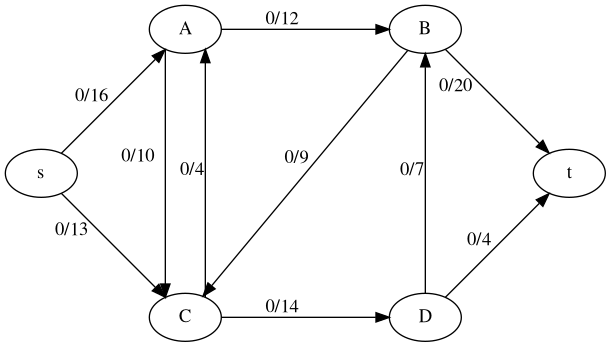
\includegraphics[width=0.5\textwidth]{img/init.png}
		\caption{Initial state}
	\end{figure}

	The first augmenting path we use is s $\rightarrow$ A $\rightarrow$ B $\rightarrow$ t, which has a residual capacity of 12. This results in a total flow of 12.

	\begin{figure}[h]
		\centering
		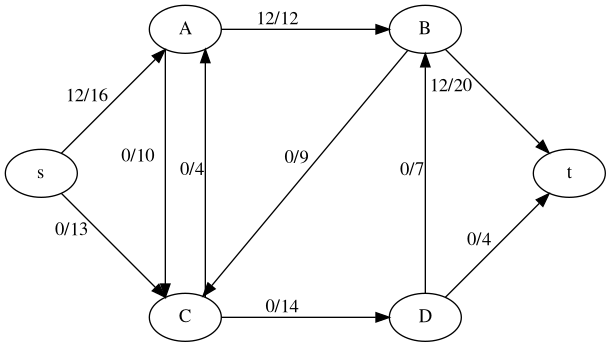
\includegraphics[width=0.5\textwidth]{img/path1.png}
		\caption{Augmenting via s $\rightarrow$ A $\rightarrow$ B $\rightarrow$ t}
	\end{figure}

	The second augmenting path we use is s $\rightarrow$ C $\rightarrow$ D $\rightarrow$ t, which has a residual capacity of 4. This results in a total flow of 16.

	\begin{figure}[h]
		\centering
		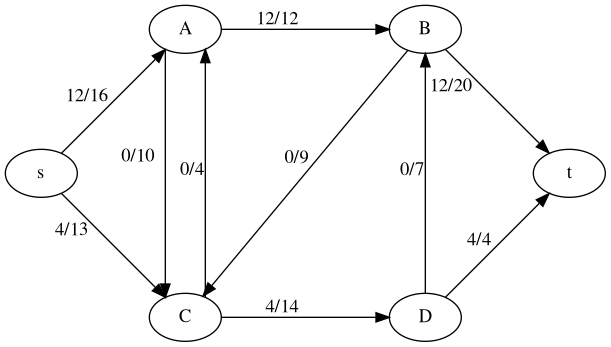
\includegraphics[width=0.5\textwidth]{img/path2.png}
		\caption{Augmenting via s $\rightarrow$ C $\rightarrow$ D $\rightarrow$ t}
	\end{figure}

	The third augmenting path we use is s $\rightarrow$ C $\rightarrow$ D $\rightarrow$ B $\rightarrow$ t, which has a residual capacity of 7. This results in a total flow of 23.

	\begin{figure}[h]
		\centering
		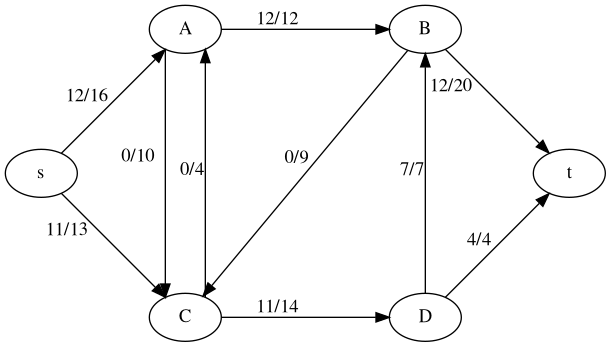
\includegraphics[width=0.5\textwidth]{img/path3.png}
		\caption{Augmenting via s $\rightarrow$ C $\rightarrow$ D $\rightarrow$ B $\rightarrow$ t}
	\end{figure}

	At this point, we can see that the if an augmenting path existed, it would have to end with B $\rightarrow$ t as D $\rightarrow$ t is already at its maximum capacity. However, the two edges through which B could increase its flow (A $\rightarrow$ B and D $\rightarrow$ B) are already at maximum capacity. Therefore, no augmenting path exists. 
	Since we can not find another augmenting path, the maximum flow through this network is 23.

	\item Edmonds–Karp algorithm

\end{enumerate}

\end{document}
